\documentclass[../main.tex]{subfiles}
\begin{document}
\part*{Results}

The Results section of the document showcases the functionality of the AWS-based image classification system. The user interface of the web application comprises a simple web page that allows users to upload any number of images for classification as shown in Figure~\ref{fig:ui} . The UI has a "Choose file" button that enables users to select the image files to be uploaded, and an "Upload" button to upload them to the AWS services.
\begin{figure}[h!]
\centering

\includegraphics[scale=0.36]{images/ui.png}
\caption{User Interface.}
\label{fig:ui}
\end{figure}

Upon clicking the "Upload" button, the web application automatically creates EC2 instances based on the number of uploaded images. Figure~\ref{fig:ins} displays the number of instances running based on the number of images uploaded. This dynamic scaling of the App-tier instances ensures that the system can handle a large number of requests efficiently.
\begin{figure}[h!]
\centering
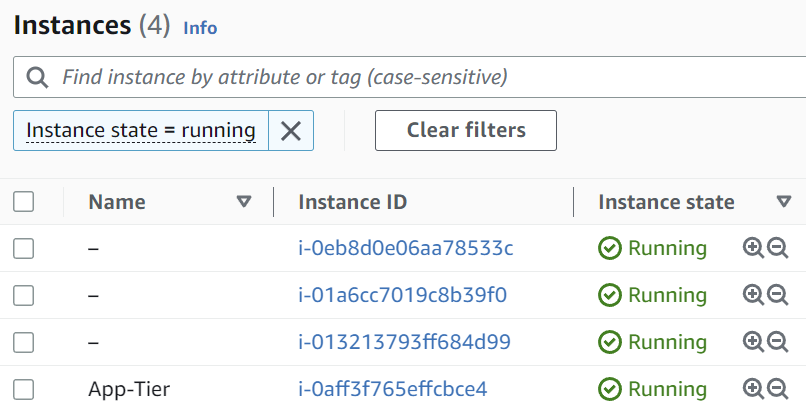
\includegraphics[scale=0.65]{images/ins.png}
\caption{If the number of uploaded images is over 15, 17 instances will run, otherwise, the app-tier instance and the number of messages will run for less than 15 uploaded images.}
\label{fig:ins}
\end{figure}

After the images have been processed, the system returns the classification results in the form of key-value pairs. The screenshot of Figure~\ref{fig:op} displays the results beneath the "Upload" button on the same webpage. Each image is labeled with its corresponding class and displayed in the format: \verb|test_0.JPEG, hair_spray|. This user-friendly interface enables users to quickly and easily classify multiple images with high accuracy, thanks to the use of a pre-trained ResNet model.
\begin{figure}[h!]
\centering
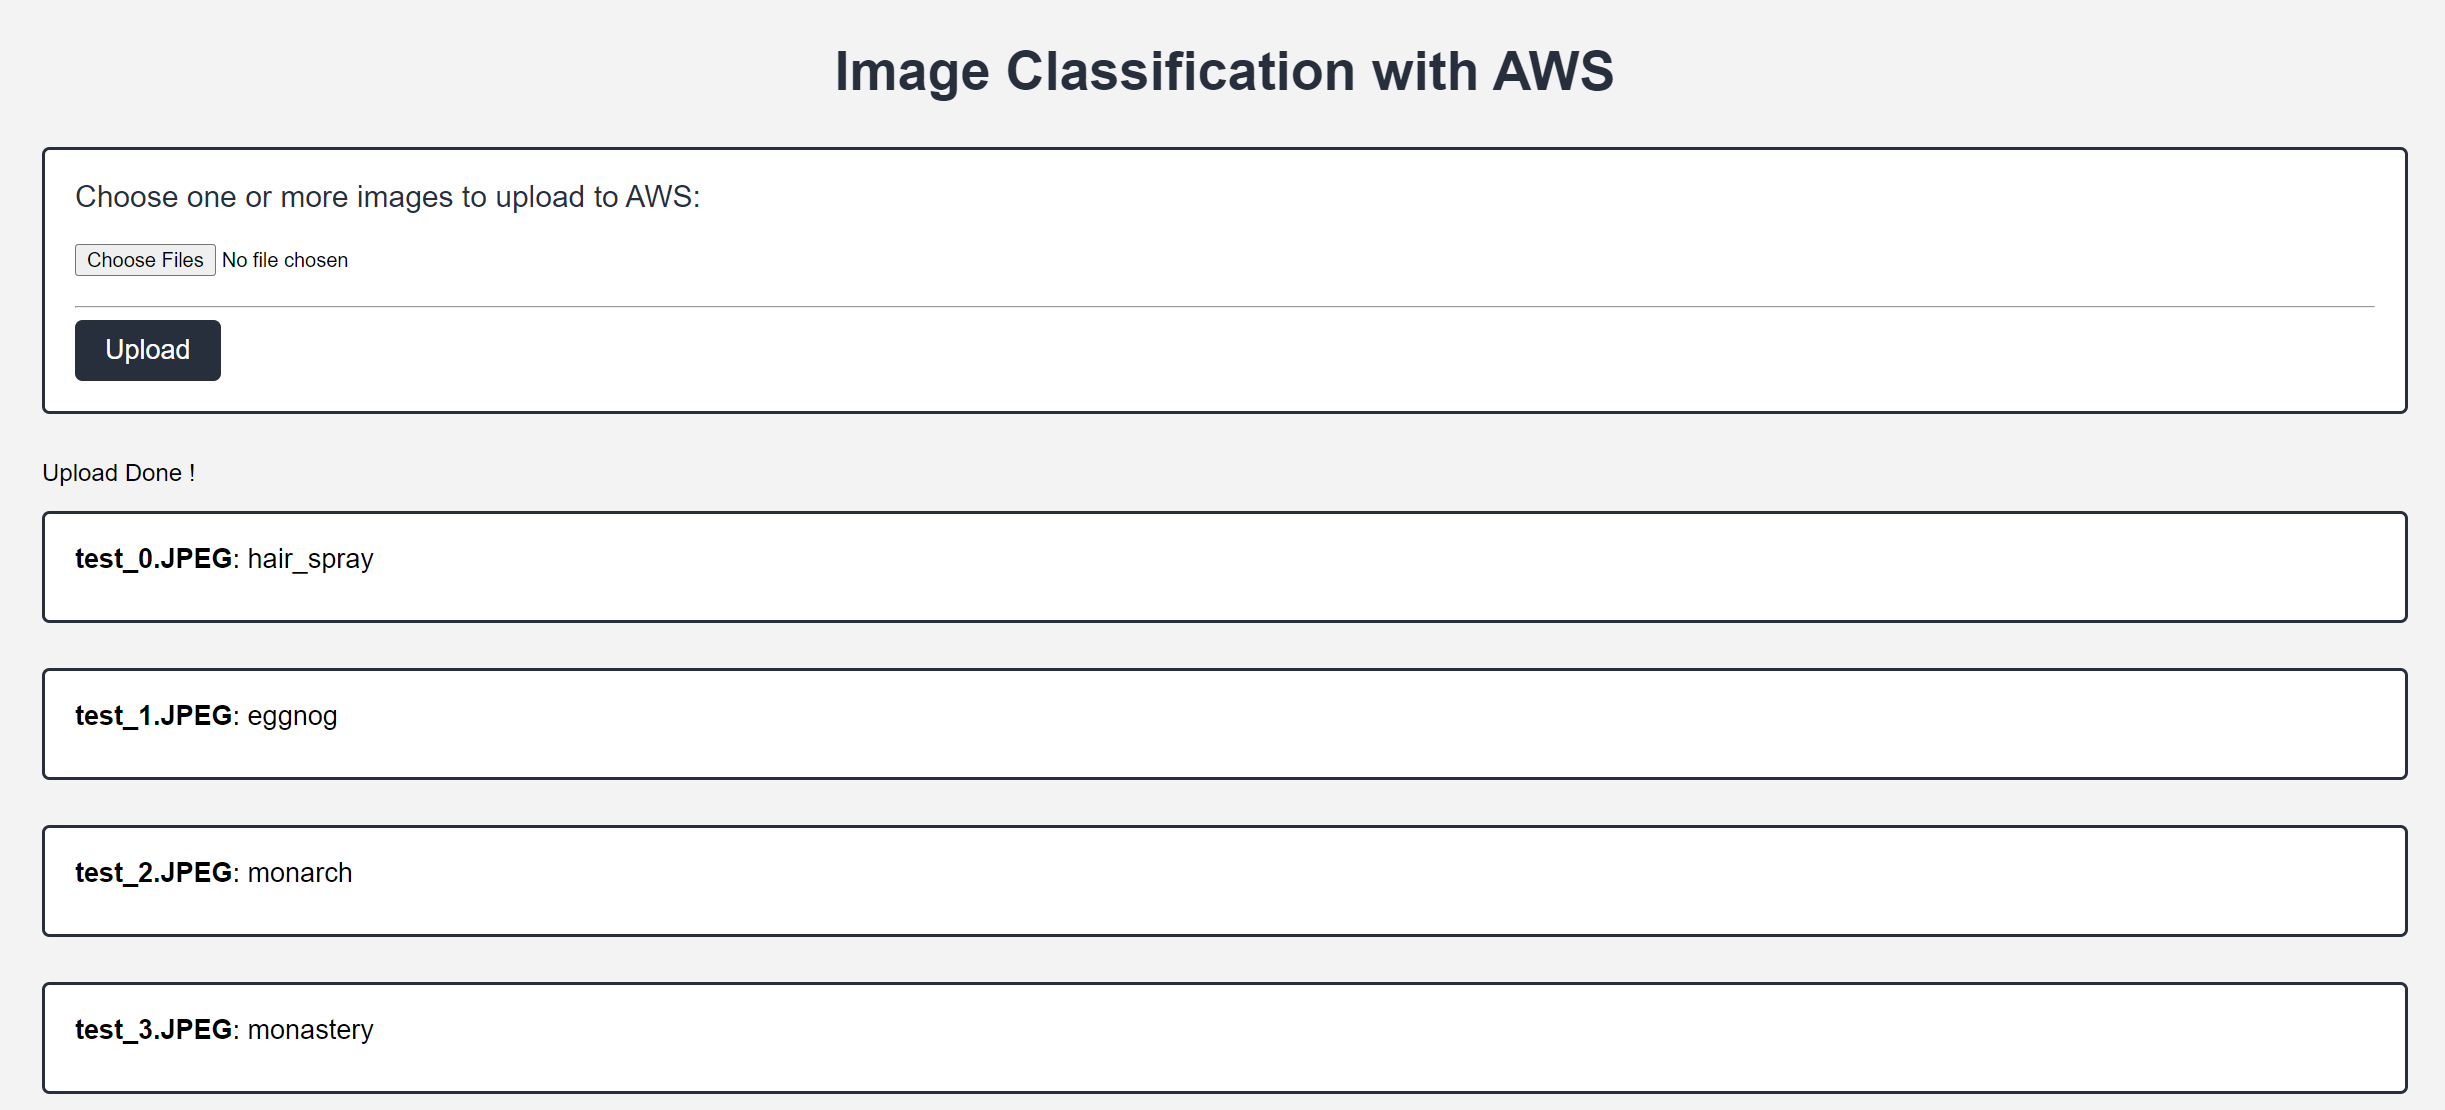
\includegraphics[scale=0.36]{images/output.png}
\caption{Sample output displayed on the UI.}
\label{fig:op}
\end{figure}

\subsection*{Evaluation based on Metrics:}
In order to evaluate the performance of the system, we measured the response time and boot time for entire processing of the system and booting time of ec2 instance. 
\newpage

\begin{itemize}
    \item Response time for uploading and classifying images was measured using the Python 'time' module.
    \item \textbf{Medium sized images ($\approx 80$ kb):}
    \begin{itemize}
        \item 20 images took an average of 230.15 seconds to display results on the webpage.
        \item 30 images took an average of 215.67 seconds to display results on the webpage.
        \item Medium sized images were classified perfectly.
    \end{itemize}        
    \item \textbf{Lower sized images ($<$2 kb):}
    \begin{itemize}
        \item 27 images took approximately 600 seconds to upload.
        \item Lower sized images did not get accurate classification results.
    \end{itemize}
    \item \textbf{Issues faced while uploading images:}
    \begin{itemize}
        \item Memory errors were encountered while uploading 60 images.
        \item Looping occurred after the 26th image while uploading 40 images.
        \item Investigation needed to determine the maximum number of images that can be uploaded at a time - To determine root cause at varying levels.
    \end{itemize}
    \item Average boot time for App-Tier's EC2 instance (excluding the delay of 30 seconds) was calculated from multiple test runs:
    \begin{itemize}
        \item Average boot time was found to be 71.53 seconds based on the results from the several test runs.
    \end{itemize}
\end{itemize}


% The total time taken to print the results on the webpage is calculated by measuring the time difference between two events: the first event is the time when the user clicks the upload button to initiate the image classification process, and the second event is the time it takes to display the results on the webpage. This time difference is calculated using the Python \verb|'time'| module, which provides functions to measure time in seconds. By subtracting the start time from the end time, we can determine the total time taken to print the results on the webpage.

\end{document}
\clearpage